\documentclass{report}
\usepackage{graphicx}
\usepackage[Export]{adjustbox}
\usepackage{hyperref}
\usepackage{enumitem}
\usepackage{amsmath}
\usepackage[makeroom]{cancel}
\usepackage{xcolor}
\usepackage{titlesec}
\usepackage{chngcntr}
\usepackage{accents}
\usepackage{pgfplots}
\usepackage{setspace}
\usepackage{tikz}
\usetikzlibrary{arrows}
\pgfplotsset{compat=1.18}

\hypersetup{
    colorlinks=true,
    linkcolor=blue,
    filecolor=magenta,      
    urlcolor=cyan,
    pdftitle={Latihan Soal PSAJ Matematika},
    pdfpagemode=FullScreen,
    }
\urlstyle{same}

\newcommand{\options}[5]{
\begin{enumerate}[label=\alph*.]
	\item #1
	\item #2
	\item #3
	\item #4
	\item #5
\end{enumerate}
}


\newcommand{\pemb}{ \textbf{Pembahasan} \\}


\titleformat{\chapter}[display]
  {\normalfont\bfseries}{}{0pt}{\Large}

\counterwithin*{equation}{section}
\counterwithin*{equation}{chapter}

\begin{document}

\chapter{Eksponen}

\section*{Sifat Eksponen}

\begin{equation}
\label{ex_mult}
a^{n} \cdot a^{m} = a^{n+m} 
\end{equation}

\begin{equation}
\label{ex_div}
\frac{a^{n}}{a^{m}} = a^{n-m} 
\end{equation}

\begin{equation}
\label{ex_pow}
(a^n)^m = a^{nm}
\end{equation}

\begin{equation}
\label{ex_neg}
a^{-n}=\frac{1}{a^n}
\end{equation}

\begin{equation}
\label{ex_frac}
a^{\frac{n}{m}}=\sqrt[n]{a^m}
\end{equation}

\begin{equation}
\label{ex_div_pow}
\left(\frac{a}{b}\right)^{n} = \frac{a^{n}}{b^{n}}
\end{equation}

\begin{enumerate}
% No. 1
\item
Bentuk sederhana dari $\left(\frac{x^{2}y^{3}z^{-1}}{x^{-3}y^{-4}z^{3}}\right)^3$ adalah \ldots
\options
{$\frac{x^{15} y^{21}}{z^6}$}
{$\frac{x^{15} y^{21}}{z^8}$}
{\textcolor{red}{{$\frac{x^{15} y^{21}}{z^{12}}$}}}
{$\frac{x^{15} y^{21}}{z^{10}}$}
{$\frac{x^{15} y^{21}}{z^{14}}$}

\pemb

Menggunakan sifat eksponen \ref{ex_pow}
\[
	\left(\frac{x^{2}y^{3}z^{-1}}{x^{-3}y^{-4}z^{3}}\right)^3 = \frac{x^{6}y^{9}z^{-3}}{x^{-9}y^{-12}z^{9}}
\]

Menggunakan sifat eksponen \ref{ex_neg}
\[
	\frac{x^{6}y^{9}z^{-3}}{x^{-9}y^{-12}z^{9}} =
	\frac{x^{6}y^{9}x^{9}y^{12}}{z^{3}z^{9}}
\]

Menggunakan sifat eksponen \ref{ex_mult}
\[
	\frac{x^{6}y^{9}x^{9}y^{12}}{z^{3}z^{9}} = 
	\frac{x^{15} y^{21}}{z^{12}} \text{(C)}
\]


% No. 2
\item
Nilai dari $\left(\frac{1}{8}\right)^{\frac{-2}{3}}+32^{\frac{2}{5}}+27^{\frac{2}{3}}$ adalah \ldots
\options
{8}
{9}
{10}
{14}
{\textcolor{red}{17}}

\pemb

Menggunakan sifat eksponen \ref{ex_pow}
\[
	\left(\frac{1}{8}\right)^{\frac{-2}{3}}+32^{\frac{2}{5}}+27^{\frac{2}{3}} = 
	\sqrt[3]{\left(\frac{1}{8}\right)^{-2}}+\sqrt[5]{32^{2}}+\sqrt[3]{27^{2}}
\]

Menggunakan sifat eksponen \ref{ex_div_pow}
\[
	\sqrt[3]{\left(\frac{1}{8}\right)^{-2}}+\sqrt[5]{32^{2}}+\sqrt[3]{27^{2}} =
	\sqrt[3]{\frac{1^{-2}}{8^{-2}}}+\sqrt[5]{32^{2}}+\sqrt[3]{27^{2}}	
\]

Menggunakan sifat eksponen \ref{ex_neg} \\
\begin{align*}
	\sqrt[3]{\frac{1^{-2}}{8^{-2}}}+\sqrt[5]{32^{2}}+\sqrt[3]{27^{2}} 
	&= \sqrt[3]{\frac{\frac{1}{1^{2}}}{\frac{1}{8^{2}}}}+\sqrt[5]{32^{2}}+\sqrt[3]{27^{2}}\\
	&= \sqrt[3]{64}+\sqrt[5]{32^{2}}+\sqrt[3]{27^{2}}\\
	&= 4 + 2^2 + 3^2 \\
	&= 4 + 4 + 9 \\
	&= 17  \text{(E)}
\end{align*}

% No. 3
\item
Hasil dari $2\sqrt{48}-4\sqrt{75}+3\sqrt{12}$ = \ldots
\options
{$18\sqrt{3}$}
{$12\sqrt{3}$}
{$3\sqrt{3}$}
{$-3\sqrt{3}$}
{\textcolor{red}{$-6\sqrt{3}$}}
\pemb
Karena semua pilihan memiliki $\sqrt{3}$, maka akar-akar disederhanakan ke bentuk $x\sqrt{3}$
\begin{align*}
	2\sqrt{48}-4\sqrt{75}+3\sqrt{12} 
	&= 2\sqrt{16.3}-4\sqrt{25.3}+3\sqrt{4.3} \\
	&= 2.4\sqrt{3}-4.5\sqrt{3}+3.2\sqrt{3} \\
	&= 8\sqrt{3}-20\sqrt{3}+6\sqrt{3} \\
	&= -6\sqrt{3} \text{(E)}
\end{align*}

% No. 4
\item
Bentuk sederhana dari $\frac{3\sqrt{5}}{3\sqrt{5}+\sqrt{3}}$ adalah \ldots
\options
{$\frac{15-\sqrt{15}}{-14}$}
{$\frac{15+\sqrt{15}}{-14}$}
{\textcolor{red}{$\frac{15-\sqrt{15}}{14}$}}
{$\frac{12-\sqrt{15}}{-14}$}
{$\frac{12-\sqrt{15}}{15}$}
\pemb
Rasionalkan akar dengan cara mengalikan pembilang dan penyebut dengan pasangan sekawan dari penyebut
\begin{align*}
	\frac{3\sqrt{5}}{3\sqrt{5}+\sqrt{3}} \cdot \frac{3\sqrt{5}-\sqrt{3}}{3\sqrt{5}-\sqrt{3}}
	&= \frac{3\sqrt{5}\left(3\sqrt{5}-\sqrt{3}\right)}{45-3} \\
	&= \frac{\cancel{3}\sqrt{5}\left(3\sqrt{5}-\sqrt{3}\right)}{\cancelto{14}{42}} \\
	&= \frac{\sqrt{5}\left(3\sqrt{5}-\sqrt{3}\right)}{14} \\
	&= \frac{3.5-\sqrt{15}}{14} \\
	&= \frac{15-\sqrt{15}}{14} \text{(C)}
\end{align*}

\chapter{Logaritma}
\section*{Sifat logaritma}

\begin{equation}
\label{log_add}
{}^a\log_{b} + {}^a\log_{c} = {}^{a}\log_{b.c}
\end{equation}

\begin{equation}
\label{log_sub}
{}^a\log_{b} - {}^a\log_{c} = {}^{a}\log_{\frac{b}{c}}
\end{equation}

\begin{equation}
\label{log_chain}
{}^a\log_{b} . {}^b\log_{c} . {}^c\log_{d} = {}^a\log_{d}
\end{equation}

\begin{equation}
\label{log_ext}
{}^{{a}^{m}}\log_{b^{n}} = \frac{n}{m}{}^a\log_{ b}
\end{equation}

\begin{equation}
\label{log_one}
{}^{a}\log_{a} = 1
\end{equation}

% No. 5
\item
Nilai dari ${}^{16}\log_{81}.{}^{3}\log_{125}.{}^{5}\log_{32}$ adalah \ldots
\options
{8}
{10}
{\textcolor{red}{15}}
{28}
{32}
\pemb

\begin{align*}
	{}^{16}\log_{81}.{}^{3}\log_{125}.{}^{5}\log_{32} = {}^{2^{4}}\log_{3^{4}}.{}^{3^1}\log_{5^3}.{}^{5^1}\log_{2^5}
\end{align*}
Menggunakan sifat logaritma \ref{log_ext}
\begin{align*}
	{}^{2^{4}}\log_{3^{4}}.{}^{3^1}\log_{5^3}.{}^{5^1}\log_{2^5} = \frac{4}{4}\cdot\frac{3}{1}\cdot\frac{5}{1}{}^{2}\log_{3}.{}^{3}\log_{5}.{}^{5}\log_{2}
\end{align*}
Menggunakan sifat logaritma \ref{log_chain}
\begin{align*}
	15{}^{2}\log_{3}.{}^{3}\log_{5}.{}^{5}\log_{2} 
	&= 15 {}^{2}\log_{2} 
\end{align*}
Menggunakan sifat logaritma \ref{log_chain}
\begin{align*}
	15 {}^{2}\log_{2} 
	&= 15.1 \\
	&= 15 \text{(C)}
\end{align*}

\item
Nilai dari ${}^{3}\log_{81}+{}^{5}\log_{300}-{}^{5}\log_{12}+{}^{2}\log_{\frac{1}{64}}$ adalah \ldots
\options
{-2}
{-1}
{\textcolor{red}0}
{1}
{6}
\pemb
Menggunakan sifat logaritma \ref{log_sub}
\begin{align*}
	{}^{3}\log_{81}+{}^{5}\log_{300}-{}^{5}\log_{12}+{}^{2}\log_{\frac{1}{64}} 
	&= {}^{3}\log_{81}+{}^{5}\log_{\frac{300}{12}}+{}^{2}\log_{\frac{1}{64}} \\
	&= {}^{3}\log_{81}+{}^{5}\log_{25}+{}^{2}\log_{\frac{1}{64}} \\
	&= {}^{3}\log_{3^4}+{}^{5}\log_{5^2}+{}^{2}\log_{2^{-6}} 
\end{align*}
Menggunakan sifat logaritma \ref{log_one}
\begin{align*}
	{}^{3}\log_{3^4}+{}^{5}\log_{5^2}+{}^{2}\log_{2^{-6}} 
	&= 4 + 2 - 6 \\
	&= 0 \text{(C)}
\end{align*}

\chapter{Persamaan Kuadrat}

% No. 7
\item
Akar -akar penyelesaian persamaan kuadrat $x^2-x-20=0$ adalah \ldots
\options
{-4 dan -5}
{4 dan -5}
{\textcolor{red}{-4 dan 5}}
{2 dan -10}
{2 dan 10}
\pemb
Faktorkan Persamaan Kuadrat
\begin{align*}
    x^2-x-20&=0 \\
    (x+4)(x-5)&=0
\end{align*}
\begin{center}
\begin{tabular}{c c c}
	\parbox{3cm}{
		\begin{align*}
		x+4&=0 \\
		x&=-4
		\end{align*}
	} & \parbox{0.8cm}{atau} &
	\parbox{3cm}{
		\begin{align*}
		x-5&=0 \\
		x&=5
		\end{align*}
	}
\text{(C)}
\end{tabular}
\end{center}

% No. 8
\item Perhatikan grafik berikut! \\
\begin{tikzpicture}
	\begin{axis}[ymin=-10, ymax=10, xmin=-10, xmax=10,
		axis line style={->},
		axis lines=middle,
		xlabel=$x$,
		ylabel=$y$,
		domain=-1:7
		]
	\addplot+[<->,mark=none,line width=1pt, samples=100]{x^2-6*x+5};
	\addplot [blue, mark = *, nodes near coords=\textcolor{black}{(3, -4)},every node near coord/.style={anchor=90}] coordinates {(3,-4)};
	\end{axis}
\end{tikzpicture}
Persamaan grafik fungsi kuadrat tersebut adalah \ldots
\options
{$y = x^2-5x+6$}
{$y = x^2-6x+5$}
{$y = x^2+6x-5$}
{$y = x^2-5x-6$}
{$y = x^2-6x+5$}
\pemb
Graf tersebut berpotongan dengan sumbu x pada titik \text{(1, 0)} dan \text{(5, 0)}
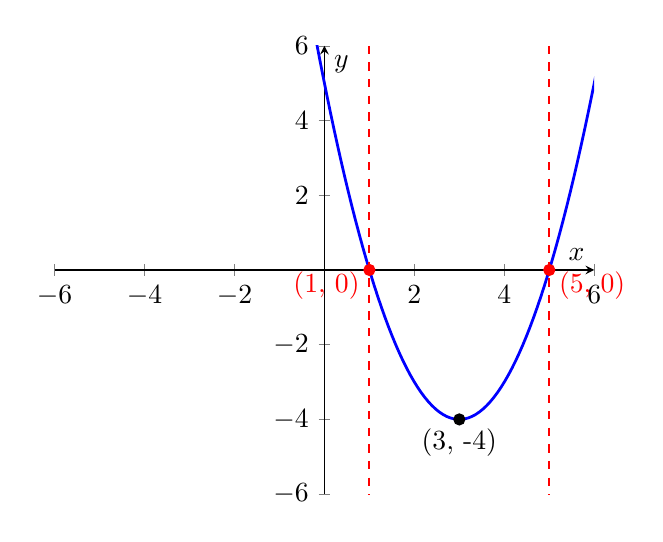
\begin{tikzpicture}
	\begin{axis}[ymin=-6, ymax=6, xmin=-6, xmax=6,
		axis line style={->},
		axis lines=center,
		xlabel=$x$,
		ylabel=$y$,
		domain=-1:7
		]
	\addplot+[<->,mark=none,line width=1pt, samples=100]{x^2-6*x+5};
	\addplot [black, mark = *, nodes near coords=\text{(3, -4)},every node near coord/.style={anchor=90}] coordinates {(3,-4)};
	\addplot[thick, samples=50, dashed,red] coordinates {(5,10)(5,-15)};
	\addplot [red, mark = *, nodes near coords=\text{(5, 0)},every node near coord/.style={anchor=160}] coordinates {(5, 0)};
	\addplot[thick, samples=50, dashed,red] coordinates {(1,10)(1,-15)};
	\addplot [red, mark = *, nodes near coords=\text{(1, 0)},every node near coord/.style={anchor=20}] coordinates {(1, 0)};
	\end{axis}
\end{tikzpicture}
\[
	x_{1} = 1 \text{ dan } x_{2} = 5
\]
Mencari persamaan kuadrat
\begin{align*}
	y 
	&= (x-x_{1})(x-x_{2}) \\
	&= (x-1)(x-5) \\
	&= x^2-6x+5 \text{ (E)}
\end{align*}

\chapter{Matriks}

\section{Istilah-istilah dalam matriks}
\textit{\textbf{TODO}}
\section{Operasi Matriks}

Penjumlahan Matriks
\begin{equation}
\label{max_add}
	\begin{bmatrix}
		a & b \\
		c & d \\
	\end{bmatrix}
	+
	\begin{bmatrix}
		e & f \\
		g & h \\
	\end{bmatrix}
	= 
	\begin{bmatrix}
		a + e & b + f \\
		c + g & d + h \\
	\end{bmatrix}
\end{equation}

Pengurangan Matriks
\begin{equation}
\label{max_sub}
	\begin{bmatrix}
		a & b \\
		c & d \\
	\end{bmatrix}
	-
	\begin{bmatrix}
		e & f \\
		g & h \\
	\end{bmatrix}
	= 
	\begin{bmatrix}
		a - e & b - f \\
		c - g & d - h \\
	\end{bmatrix}
\end{equation}


Transposisi Matriks
\begin{equation}
\label{max_transp}
    A = \begin{bmatrix}
		a & b & c\\
		d & e & f\\
	\end{bmatrix}
	\to
	A^{T} = \begin{bmatrix}
		a & d \\
		b & e \\
		c & f \\
	\end{bmatrix}
\end{equation}

Invers Matrix Ordo 2 x 2
\begin{equation}
\label{max_transp}
    A = \begin{bmatrix}
		a & b & c\\
		d & e & f\\
	\end{bmatrix}
	\to
	A^{T} = \begin{bmatrix}
		a & d \\
		b & e \\
		c & f \\
	\end{bmatrix}
\end{equation}
\begin{doublespace}
    \item Diketahui matriks $ P=
	    \begin{bmatrix}
		    x+2y & 3 \\
		    2x-y & -6 \\
	    \end{bmatrix}
	    $  dan $Q=
	    \begin{bmatrix}
		    3 & -2 \\
		    2 & -1 \\
	    \end{bmatrix}
	    $. Jika $P^{T} = Q$ maka nilai $4x-3y$ adalah \ldots
\end{doublespace}


\end{enumerate}
\end{document}
